%%%%%%%%%%%%%%%%%%%%%%%%%%%%%%%%%%%%%%%%%%%%%%%%%%%%%%%%%%%%%%%%%%%%%%%%%%%%%%%%%%%
%% This project aims to create the UFC template for presentation.                %%
%% author: NGUYEN Tan Sy - Doctoral student in Computer Science (MDCC)           %%
%% contacts:                                                                     %%
%%    e-mail: tansyab1@gmail.com                                                 %%
%%                                                                               %%
%%%%%%%%%%%%%%%%%%%%%%%%%%%%%%%%%%%%%%%%%%%%%%%%%%%%%%%%%%%%%%%%%%%%%%%%%%%%%%%%%%%
\documentclass{libs/ufc_format}
% Inserting the preamble file with the packages
%%%%%%%%%%%%%%%%%%%%%%%%%%%%%%%%%%%%%%%%%%%%%%%%%%%%%%%%%%%%%%%%%%%%%
%% This file contains the packages that can be used in the beamer. %%
%%%%%%%%%%%%%%%%%%%%%%%%%%%%%%%%%%%%%%%%%%%%%%%%%%%%%%%%%%%%%%%%%%%%%
% Package to fonts family
\usepackage[T1]{fontenc}
% Package to accentuation
\usepackage[utf8]{inputenc}
% Package to Portuguese language
\usepackage[english]{babel}
% Package to Figures
\usepackage{graphicx}
% Package to the colors
\usepackage{color}
% Package to the colors
\usepackage{xcolor}
% Packages to math symbols and expressions
\usepackage{amsfonts, amssymb, amsmath}
% Package to multiple lines and columns in table
\usepackage{multirow, array} 
% Package to create pseudo-code
% For more detail of this package: http://linorg.usp.br/CTAN/macros/latex/contrib/algorithm2e/doc/algorithm2e.pdf
\usepackage{algorithm2e}
% Package to insert code
\usepackage{listings} 
\usepackage{keyval}
% Package to justify text
\usepackage[document]{ragged2e}
% Package to manage the bibliography
\usepackage[backend=biber, style=numeric, sorting=none]{biblatex}
% Package to facilities quotations
\usepackage{csquotes}
% Package to use multicols
\usepackage{multicol}
\usepackage{tikz}
\usepackage{times}
\usepackage{amsmath,adjustbox}
\usepackage{verbatim}
\usetikzlibrary{calc, arrows, shapes}
\usepackage[beamer,customcolors]{hf-tikz}
\usepackage{transparent}

\renewcommand{\familydefault}{\sfdefault}
\newcommand{\tikzmark}[1]{\tikz[overlay,remember picture] \node (#1) {};}
\usepackage{lmodern}
\setbeamertemplate{bibliography item}{\insertbiblabel}
% Inserting the references file
\bibliography{references.bib}


% Title
\title[A new dataset of distortions on WCE images]{\textbf{A new dataset of distortions on Wireless Capsule Endoscopy Images for pathological ifentification}}
% Subtitle
% \subtitle{Subtítulo da Apresentação}
% Author of the presentation
\author{Tan Sy NGUYEN}
% Institute's Name
\institute[- USPN]{
    % email for contact
    \normalsize{\email{tansy.nguyen@math.univ-paris13.fr}}
    \newline
    % Department Name
    \department{LAGA, L2TI}
    \newline
    % university name
    \uspn
}
% date of the presentation
\date{\today}


%%%%%%%%%%%%%%%%%%%%%%%%%%%%%%%%%%%%%%%%%%%%%%%%%%%%%%%%%%%%%%%%%%%%%%%%%%%%%%%%%%
%% Start Document of the Presentation                                           %%               
%%%%%%%%%%%%%%%%%%%%%%%%%%%%%%%%%%%%%%%%%%%%%%%%%%%%%%%%%%%%%%%%%%%%%%%%%%%%%%%%%%
\begin{document}
% insert the code style
%%%%%%%%%%%%%%%%%%%%%%%%%%%%%%%%%%%%%%%%%%%%%%%%%%%%%%%%%%%%%%%%%%%%%%%%%%%%%%%%%%%
%% This file contains the style of the codes show in slides.                     %%
%% The package used is listings, but it possible to used others.                 %%
%%%%%%%%%%%%%%%%%%%%%%%%%%%%%%%%%%%%%%%%%%%%%%%%%%%%%%%%%%%%%%%%%%%%%%%%%%%%%%%%%%%

% color used in the code style
\definecolor{codegreen}{rgb}{0,0.6,0}
\definecolor{codegray}{rgb}{0.5,0.5,0.5}
\definecolor{codepurple}{rgb}{0.58,0,0.82}
\definecolor{codebackground}{rgb}{0.95,0.95,0.92}

% style of the code!
\lstdefinestyle{codestyle}{
    backgroundcolor=\color{codebackground},   
    commentstyle=\color{codegreen},
    keywordstyle=\color{magenta},
    numberstyle=\tiny\color{codegray},
    stringstyle=\color{codepurple},
    basicstyle=\ttfamily\footnotesize,
    frame=single,
    breakatwhitespace=false,         
    breaklines=true,                 
    captionpos=b,                    
    keepspaces=true,                 
    numbers=left,                    
    numbersep=5pt,                  
    showspaces=false,                
    showstringspaces=false,
    showtabs=false,                  
    tabsize=2,
    title=\lstname 
}

\lstset{style=codestyle}


%% ---------------------------------------------------------------------------
% First frame (with tile, subtitle, ...)
\begin{frame}{}
    \maketitle
\end{frame}

%% ---------------------------------------------------------------------------
% Second frame
\begin{frame}{Overview}
    % \begin{multicols}{2}
        \tableofcontents
    % \end{multicols}
\end{frame}

%% ---------------------------------------------------------------------------
% This presentation is separated by sections and subsections
\section{Objectives}
\begin{frame}{Objectives}
    % enumeration
    The main objective of the project is to develop a smart system for:
    \begin{itemize}
        \item Identify the pathological finding on wireless capsule endoscopy (WCE) images
        \begin{itemize}
            \item Including a pre-processing module that aims at improving the quality of the acquired images
            \item Develop a set of image quality enhancement solutions based on kinds of distortion
        \end{itemize}
        
        
    \end{itemize}

    \vspace{0.2cm}

     There are \example{many kinds of distortion} $\&$ in \emph{different levels}
\end{frame}

%% ---------------------------------------------------------------------------
\subsection{Context}

\begin{frame}{Context}
\begin{alertblock}{Alert}
         Colorectal cancer is a major health problem.
    \end{alertblock}
    \pause
\begin{block}{Example}
        In 2018, the Colorectal cancer (CRC) is the third (second respectively) leading cause of cancer death in the world (France, respectively).\footnote[frame]{\tiny Bray F, Ferlay J, Soerjomataram I, Siegel RL, Torre LA, Jemal A, "Global cancer statistics 2018: GLOBOCAN estimates of \\ \hspace{0.3cm}incidence and mortality worldwide for 36 cancers in 185 countries", CA Cancer J Clin. 2018 Nov; 68(6):394-424.}$^{,}$\footnote[frame]{\tiny Santé Publique France, https://www.santepubliquefrance.fr/maladies-et-traumatismes/cancers/cancer-du-colon-rectum}
    \end{block}
\pause
    \begin{exampleblock}{Solution}
        Studies have shown that early detection can result in up to a \example{92\% survival rate for stage I of cancer.}\footnote[frame]{\tiny McKESSON, "Colorectal Cancer \& Laboratory Screening", 2018}
    \end{exampleblock}  
    
\end{frame}


%% ---------------------------------------------------------------------------
\subsection{Wireless Capsule Endoscopy}
\begin{frame}{Wireless Capsule Endoscopy}

    \alertbox{ \textbf{Traditional} endoscopy is often \textcolor{red}{unpleasant} and \textcolor{red}{uncomfortable} for the patient, can be \textcolor{red}{painful}, often requires moderate or deep sedation}
    
    \pause
    
    \successbox{\textbf{Wireless capsule endoscopy} include its \example{non-invasive} character and its ability to visualize proximal and distal parts of the intestine}
    
\end{frame}


\subsubsection{Challenges}
\begin{frame}{Challenges}
    % \textcolor{blue(pigment)}{\textbf{Challenges and Motivation}}\\[5pt]
    \begin{itemize}
        % \item Current challenges in the hospital: "\textcolor{red}{2 patients/day} and just \textcolor{violet}{4 working days}" 
        \item Some common acquisition distortions (\textbf{noise}, \textcolor{red}{\textbf{blur}}, \textcolor{violet}{\textbf{uneven illumination}}, \textcolor{blue}{\textbf{specular reflection}}) may affect the WCE based diagnosis.
    \end{itemize}


    \begin{figure}
        \centering
        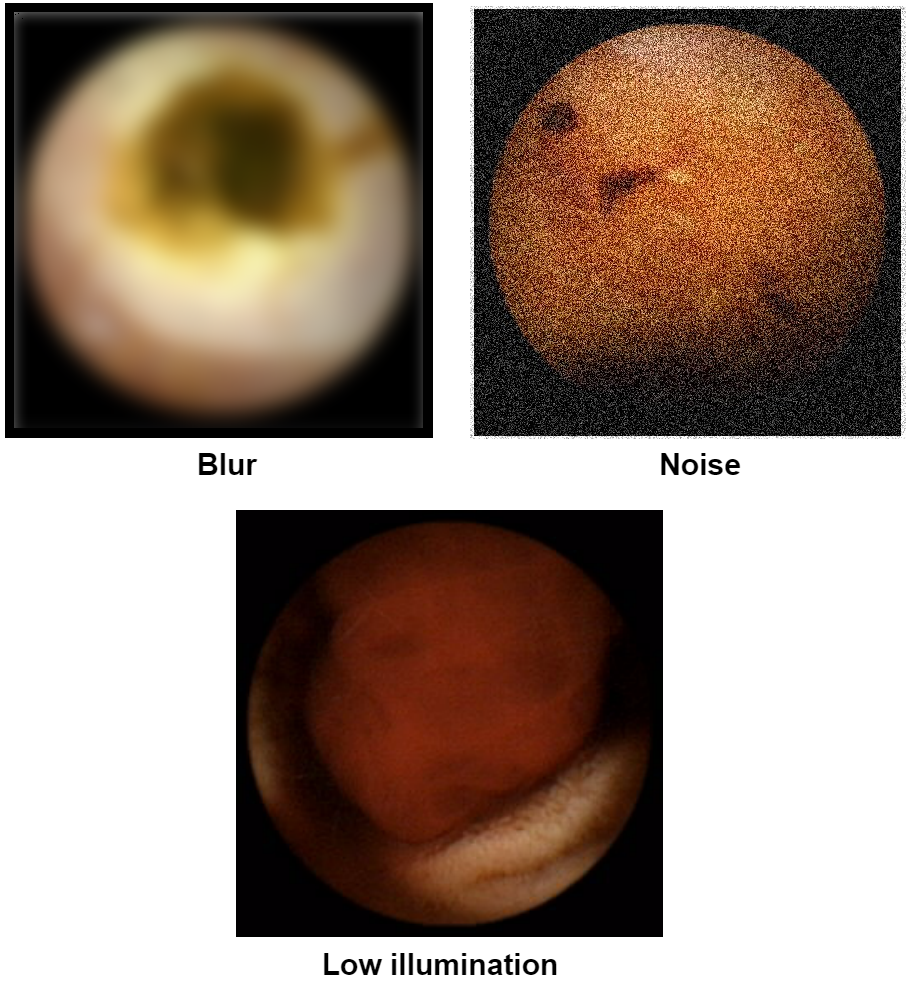
\includegraphics[scale=0.15]{libs/wcedistortions.png}
        \vspace{0.4cm}
        \caption{Illustration of some common WCE images distortions}
        \label{fig:endoscopy}
    \end{figure}

\end{frame}
\subsubsection{Solutions}
%% ---------------------------------------------------------------------------
% \subsection{Subseção III}
\begin{frame}{Algorithm}
    % \caption{Apply the approximation quality enhancement methods}
    \begin{algorithm}[H]
    
        \SetAlgoLined
        \LinesNumbered
        \SetKwInOut{Input}{input}
        \SetKwInOut{Output}{output}
        \Input{$distorted\_image$}
        \Output{$enhanced\_image$}
        $types\_distortion$ = \tikzmark{classifier}{classifier} ($distorted\_image$)\;
        \For{$type$ in $types\_distortion$}{
        $enhanced\_image$ $\gets$ \tikzmark{enhancer}{enhancer$_{type}$} ($distorted\_image$)
        }
        \Return $enhanced\_image$
        % \vspace{cao0.5cm}
        
    \end{algorithm}
    
    \pause
    \tikz[overlay,remember picture]{\draw[draw=blue,thick,fill opacity=0.2] ($(classifier)+(-0.1,0.3)$) rectangle ($(classifier)+(1.3,-0.1)$);}
    
    \tikz[overlay,remember picture]{\draw[draw=green,thick,fill opacity=0.2] ($(enhancer)+(-0.1,0.3)$) rectangle ($(enhancer)+(1.9,-0.2)$);}

    \texttt{Requirement:}
    
    Create the \tikz[remember picture]{ \node[anchor=base] (n1) {\tikzmark{classifier}{classifier}};} and \tikz[remember picture]{ \node[anchor=base] (n2) {\tikzmark{enhancer}{enhancer$_{type}$}};}\tikz[overlay,remember picture]{\draw[draw=blue,thick,fill opacity=0.2] ($(classifier)+(-0.1,0.3)$) rectangle ($(classifier)+(1.3,-0.1)$);}\tikz[overlay,remember picture]{\draw[draw=green,thick,fill opacity=0.2] ($(enhancer)+(-0.1,0.3)$) rectangle ($(enhancer)+(1.9,-0.2)$);}
    \pause by using \example{learning - based} method 
    
    \pause 
    \vspace{0.5cm}
    \tikz[remember picture]{ \node[fill=green!20,anchor=base] (t1) {Creating a dataset is the \emph{most important} thing to do};}
    \begin{tikzpicture}[remember picture,overlay]   %% use here too
        \path[draw=magenta,thick,->]<1-> (n1) to [bend right] (t1);
        \path[draw=magenta,thick,->]<2-> (n2) to [bend left] (t1);
\end{tikzpicture}

\end{frame}

% %% ---------------------------------------------------------------------------

% \begin{frame}{Inserindo Algoritmos}
%     \lstset{language=Python}
%     \lstinputlisting[language=Python]{code/main.py}
% \end{frame}

% %% ---------------------------------------------------------------------------
% \begin{frame}{Inserindo Algoritmos}
%     \lstinputlisting[language=C]{code/source.c}
% \end{frame}

% %% ---------------------------------------------------------------------------
% \begin{frame}{Inserindo Algoritmos}
%     \lstinputlisting[language=Java]{code/helloworld.java}
% \end{frame}

% %% ---------------------------------------------------------------------------
% \begin{frame}{Inserindo Algoritmos}
%     \lstinputlisting[language=HTML]{code/index.html}
% \end{frame}

% %% ---------------------------------------------------------------------------
% % This frame show an example to insert multicolumns
\section{Existing datasets}
\subsection{Existing GI datasets}
\begin{frame}{Existing datasets}
  \begin{table}
\caption{An overview of existing GI datasets.}
\begin{adjustbox}{width=\textwidth}
\begin{tabular}{|l|l|l|}
\hline
\rowcolor[HTML]{FFFFFF} 
\textbf{Dataset}                                     & \textbf{Findings}                                                                                        & \textbf{Size}                     \\ \hline
CVC-356 \cite{Bernal2012TowardsAP}                                             & Polyps                                                                                                   & 356 images                       \\ \hline
CVC-ClinicDB (also named CVC-612) \cite{Bernal2015WMDOVAMF}                    & Polyps                                                                                                   & 612 images                      \\ \hline
CVC-VideoClinicDB (also named CVC-12k) \cite{Bernal2012TowardsAP}              & Polyps                                                                                                   & 11954 images                    \\ \hline
CVC-ColonDB \cite{Bernal2012TowardsAP}                                       & Polyps                                                                                                   & 380 images                      \\ \hline
Endoscopy Artifact detection 2019 \cite{Ali2019EndoscopyAD}                   & Endoscopic Artifacts                                                                                     & 5,138 images                      \\ \hline
ASU-Mayo polyp database  \cite{Tajbakhsh2016AutomatedPD}                            & Polyps                                                                                                   & 18,781 images                   \\ \hline
ETIS-Larib Polyp DB \cite{Silva2013TowardED}                                & Polyps                                                                                                   & 196 images                      \\ \hline
KID \cite{Koulaouzidis2017KIDPA}                                                 & Angiectasia, bleeding, inflammations, polyps                                                              & 2371 images and 47 videos         \\ \hline
GIANA 2017  \cite{Guo2019GIANAPS}                                         & Polyps \& Angiodysplasia                                                                                 & 3462 images and 38 videos         \\ \hline
GIANA 2018  \cite{Bernal2018PolypDB}                                      & Polyps \& Small bowel lesions                                                                            & 8262 images and 38 videos         \\ \hline
GASTROLAB   \cite{gastro}                                         & GI lesions                                                                                               & Some 100s of images andfew videos \\ \hline
WEO Clinical Endoscopy Atlas \cite{weo}                        & GI lesions                                                                                               & 152 images                        \\ \hline
GI Lesions in Regular Colonoscopy Data Set \cite{uci}          & GI lesions                                                                                               & 76 images                    \\ \hline
Atlas of Gastrointestinal Endoscope  \cite{as72}                & GI lesions                                                                                               & 1295 images                       \\ \hline
El salvador atlas of gastrointestinal video endoscopy \cite{as73} & GI lesions                                                                                               & 5071 video clips                  \\ \hline
Kvasir  \cite{Pogorelov2017KVASIRAM}   & \begin{tabular}[c]{@{}l@{}} Polyps, esophagitis, ulcerative colitis, Z-line,pylorus\\ cecum, dyed polyp, dyed resection margins, stool \end{tabular}& 8000 images                       \\ \hline
Kvasir-SEG   \cite{Jha2020KvasirSEGAS}                                    & Polyps                                                                                                   & 1000 images                \\ \hline
Nerthus  \cite{Pogorelov2017NerthusAB}                                            & Stool - categorization of bowel cleanliness                                                              & 21 videos                         \\ \hline
\end{tabular}
\end{adjustbox}

\end{table}
\pause
\alertbox{They are rather small, and often limited to polyps. Several of these have also lately become unavailable.\tikz[remember picture]{ \node[anchor=base] (n3) {};}}
\pause
\tikz[remember picture]{ \node[fill=green!20,anchor=base] (t3) {Using \emph{HyperKvasir} \cite{Borgli2020HyperKvasirAC} dataset};}
\begin{tikzpicture}[remember picture,overlay]   %% use here too
        \path[draw=magenta,thick,->]<1-> (n3) to [bend right] (t3);
\end{tikzpicture}
\end{frame}
\subsection{HyperKvasir dataset}
\begin{frame}{HyperKvasir dataset}
    \begin{table}[]
\caption{Overview of the data records in the HyperKvasir dataset.}
\begin{adjustbox}{width=\textwidth}    
\begin{tabular}{|l|l|l|}
\hline
\multicolumn{1}{|c|}{\textbf{Data Record}} & \multicolumn{1}{c|}{\textbf{\# Files}} & \multicolumn{1}{c|}{\textbf{Description}} \\ \hline
\tikz[remember picture]{ \node[anchor=base] (n4) {};}Labeled images                             & 10,662 images                          & 23 classes of findings                    \\ \hline
Segmented Images                           & 1,000 images                           & Segmentation masks for polyp findings     \\ \hline
Unlabeled Images                           & 99,417 images                          & Unlabeled                                 \\ \hline
\tikz[remember picture]{ \node[anchor=base] (n5) {};}Videos                                     & 374 videos                             & 30 different classes                      \\ \hline
\end{tabular}
\end{adjustbox}
\end{table}
\pause

\begin{figure}
    \centering
    \tikz[remember picture]{ \node[anchor=base] (t4) {};}
    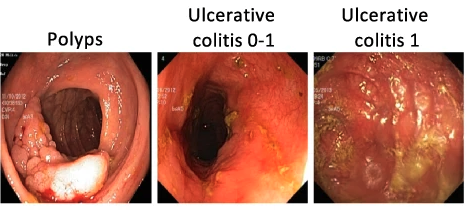
\includegraphics[scale=0.1]{libs/hyperkvasir_ex.png}
    \caption{Image examples of the various labeled classes for images and/or videos.}
\end{figure}
\begin{tikzpicture}[remember picture,overlay]   %% use here too
        \path[draw=magenta,thick,->]<1-> (n4) to [bend right] (t4);
        \path[draw=blue,thick,->]<1-> (n5) to [bend right] (t4);
\end{tikzpicture}
\end{frame}
%% ---------------------------------------------------------------------------
% This frame show an example to insert figures
\section{Our work}
\tikzset{
    vertex/.style = {
        circle,
        fill            = black,
        outer sep = 2pt,
        inner sep = 1pt,
    }
}
\begin{frame}{Ourwork}
    \begin{tikzpicture}
  % Dialectics
  \node[draw] (Original) at (0,2) {Original};
  \node[draw,fill=black,text=white] (Antidistortion) at (2.3,2) {Antidistortion};
  \node[draw,fill=gray,text=white] (Cleaner) at (1,4) {Cleaner};
  
  \draw node[vertex] (Joint) at (1,2) {};
  
 \draw[-,draw=blue] (Original) to (Joint);
  \draw[-,draw=blue] (Antidistortion) to (Joint);
  \draw[->,draw=blue] (Joint) to (Cleaner);
  \draw[->,draw=blue] (Cleaner) to[in=180,out=180] (Original);
  \node at (1.0, 1.0) {\textit{a) Clean the image}};
  \onslide<1,2>{\node (step1)  at (3,-1){   \example{Step 1} Cleaning the existing distortion in HyperKvasir dataset};}
  \pause
  \onslide<2>{
   \node (example)  at (7,2){                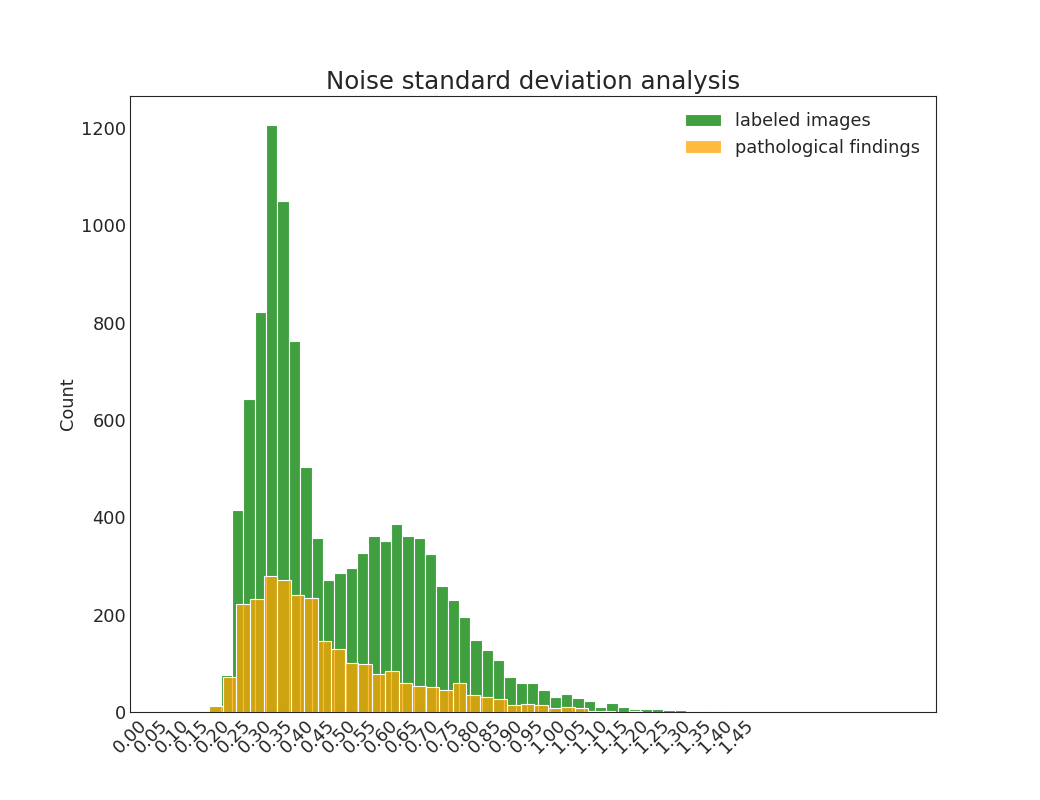
\includegraphics[width=0.5\columnwidth]{libs/sigmahist.png} };
   \draw[->,draw=red] (example) to (Cleaner);
   
   
  }
  

  \pause
  % Opposition
  \node[draw] (ArgumentA) at (5,2) {Distortion};
  \node[draw,fill=yellow] (ArgumentB) at (7.5,2) {Model};
  
  \draw[->,draw=blue] (ArgumentA) to (ArgumentB);
  
  \node at (6., 1.0) {\textit{b) Create model}};
  \onslide<3>{\node (step2)  at (3,-1){   \example{Step 2} Creating the model to generate the new artificial distortions};}
  \pause
    \onslide<4>{
    \node (old)  at (5,4){                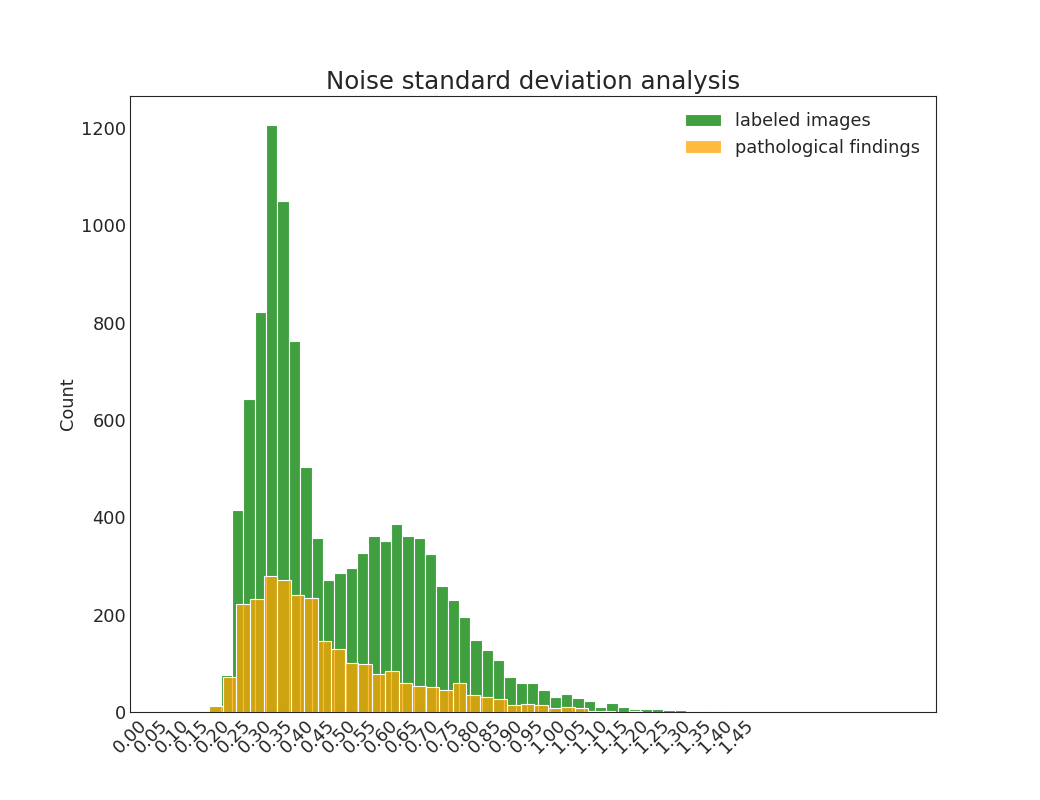
\includegraphics[width=0.2\columnwidth]{libs/sigmahist.png} };
   \draw[->,draw=yellow] (old) [bend left] to (ArgumentB);
   \node (example)  at (4,-1){   
   
\includegraphics[width=0.2\columnwidth]{libs/sb_mask.png} };
   \draw[->,draw=red] (example) [bend right] to (ArgumentB);
  }
  \pause
  % Innovation
  \node[draw,fill=black,text=white] (ArgumentA) at (2.1,-1) {Antidistortion};
  \node[draw,fill=violet,text=white] (ArgumentB) at (5.3,-1) {Opposition};
  \node[draw,fill=yellow] (ArgumentC) at (3,0) {Model};
  
  \draw node[vertex] (Joint) at (3.6,-1) {};
  
  \draw[-] (ArgumentA) to (Joint);
  \draw[-] (ArgumentB) to (Joint);
  \draw[->,draw=blue] (ArgumentC) to (Joint);
  
  \node at (3.5, -2.0) {\textit{c) Add artificial distortion}};
  \onslide<5>{\node (step2)  at (3,5){   \example{Step 3} Add the new artificial distortions to the antidistorted images};}
\end{tikzpicture}
\end{frame}

%% ---------------------------------------------------------------------------
% Reference frames
\begin{frame}[shrink=50]
    \frametitle{References}
    \printbibliography
\end{frame}

%% ---------------------------------------------------------------------------
% Final frame
\begin{frame}{}
    \centering
    \huge{\textbf{\example{Thank you for watching!}}}
    
    \vspace{1cm}
    
    \Large{\textbf{Contact:}}
    \newline
    \vspace*{0.5cm}
    \large{\email{tansy.nguyen@math.univ-paris13.fr}}
\end{frame}

\end{document}